\documentclass[a4paper,12pt]{report}
\setcounter{secnumdepth}{3} % Ensure subsubsections are numbered
\setcounter{tocdepth}{3} %per a que surtin subseccions en index (3.4.2.1 apareix amb depth 3)
\usepackage[utf8]{inputenc}
\usepackage[spanish]{babel}  % Cambia el idioma a español
\usepackage{geometry}
\usepackage{setspace}
\usepackage{titlesec}
\usepackage{graphicx}
\usepackage{hyperref} % Paquete para enlaces clicables
\usepackage{placeins} % per a les float barrier, que no es moguin les imatges.
\usepackage{titlesec}  % Paquete para personalizar títulos
\usepackage{float}  %pquete para que las figuras no se de splacen
\usepackage{listings} %para poner entronos de codigo 

% Configuración para reducir el espacio superior de los capítulos
\titleformat{\chapter}[hang]
{\normalfont\huge\bfseries} % Formato de la fuente y tamaño del capítulo
{Capítulo \thechapter}{0pt}{\huge}  % Sin espacio entre "Capítulo X" y el título
\titlespacing*{\chapter}{0pt}{-20pt}{20pt} % Ajustes de espacio antes, después, y debajo del título




\usepackage{xcolor} % Para definir colores personalizados

% Configuración del estilo para Git
\lstset{
	language=bash,                   % Usa Bash para sintaxis similar a Git
	basicstyle=\ttfamily\small,      % Texto monoespaciado y pequeño
	keywordstyle=\bfseries,          % Palabras clave en negrita
	commentstyle=\color{gray},       % Comentarios en gris
	morekeywords={git, clone, add, branch, checkout, commit, push}, % Palabras clave de Git
	showstringspaces=false           % No mostrar espacios en cadenas de texto
}



% Configuración de márgenes
\geometry{left=3cm, right=3cm, top=2.5cm, bottom=2.5cm}

% Configuración de espacios
\setstretch{1.15}


% Configuración de formato de títulos
\titleformat{\chapter}[display]
{\normalfont\bfseries\Huge}
{}{0pt}{\Huge}

\hypersetup{
	colorlinks=true,        % Colorear enlaces
	linkcolor=blue,         % Color de los enlaces internos
	urlcolor=blue,          % Color de los enlaces externos (URLs)
	pdftitle={Memoria Proyecto}, % Título del PDF
	pdfauthor={Jorge Muñoz Carrión, Santiago Sánchez Sans} % Autor
}

\begin{document}
	
	

	
	
	
	% Portada
	\begin{titlepage}
		\begin{center}

			
			\vspace*{5cm} 

			\LARGE{Creación de un dashboard para usuarios del ticket digital de Mercadona con consultas visuales a la evolución de productos habitualmente adquiridos, costes de compras por intervalos temporales y gastos por áreas de producto}
			
			\vfill
			
		\begin{flushright}
			\large{\textbf{Santiago Sánchez Sans}}
			
			\large{\textit{Ciclo formativo en desarrollo de aplicaciones web}}
			
			\large{Memoria del Proyecto de DAW}
			
			\large{IES Abastos. Curso 2024/25. Grupo 7X. XX de Junio de 2025}
			
			\large{Tutor Individual: Carlos Furones}
		\end{flushright}

			
			
			% Fecha
			
			
		\end{center}
	\end{titlepage}
	
	% Índice
	\tableofcontents
	\newpage
	
	
	
	
	
	
	
	
	% Per a conseguir que els espais apliquin solsament a les seccions no a l'index
	\begingroup
	\setlength{\parskip}{.7em}
	
	
	% Capítulos y secciones
	\chapter{Introducción}

		\section{¿Qué es el ticket digital de Mercadona?}
		
		Mercadona implementa un sistema de tickets digitales que vinculan la tarjeta de débito a un correo electrónico. Cualquier usuario del supermercado que quiera utilizar el ticket digital solamente deberá facilitar estos dos datos y el supermercado le enviará por correo electrónico los tickets de las posteriores compras hechas en cualquier establecimiento de Mercadona.
		
		Las ventajas para el usuario son evidentes: no se pierden los tickets de cara a devoluciones y el cliente del supermercado no debe esperar a la impresión del ticket.
		
		
		
		\section{Identificación de necesidades}
		\label{section:identificacionNecesidades}
		
		Los tickets de cada usuario se acumulan de forma recurrente en el correo electrónico y con un formato estructurado (los asuntos son predecibles e incluyen las fechas) y dentro de cada correo de un ticket digital se encuentra un PDF con el desglose de la compra (producto, unidades vendidas, establecimiento, etc).
		
		Esta información se acumula en el correo del usuario pero a pesar de ser una información estructurada su acceso para el usuario no es simple: no puede visualizar lo que ha gastado, ni el precio de los productos y de su evolución, ni los supermercados en los que ha comprado, ni las veces que lo ha hecho, etc.

		\section{Objetivos del proyecto} % OBLIGAT
		\label{section:objetivosProyecto}
		
		Este proyecto quiere responder a estas necesidades. Para ello se plantea la Creación de un dashboard o "cuadro de mando" front-end para que un usuario del ticket digital de Mercadona pueda visualizar la evolución de precios de los productos adquiridos, el coste promedio de sus compras por períodos temporales y sus distribuciones de gastos a partir de los tickets digitales guardados en una base de datos.
		
		
		Los \textbf{Objetivos principales} del proyecto son mostrar al usuario:

					
		\begin{itemize}
			\setlength{\itemsep}{-.5em}
			\item \textbf{Evolución de precios} (inflación) a lo largo del tiempo en los productos habitualmente comprados en el mismo establecimiento\footnote{La evolución de precios se mostrará solamente para un mismo centro de Mercadona, dado que distintos centros pueden cambiar los nombres de los productos (por ejemplo, en Cataluña…).}.
			\item \textbf{Evolución del gasto} total del usuario a lo largo del tiempo.
		\end{itemize}
		
		
		

		
		

		
		
		
		
		
		
		
		
		
		
			%IDENTIFICAR OBJECTIUS  %OBLIGAT
			%JUSTIFICAR OBJECTIUS   %OBLIGAT
			
			
	
		
	

		



		
	

		
	

		


		

		
		
		
		
	
	\chapter{Diseño del proyecto}  %OBLIGAT
	
		
				
		Para implementar los objetivos principales de los que hemos hablado en la sección \ref{section:objetivosProyecto} hemos proyectado una serie de requisitos funcionales de la aplicación.
		
		


		
		
		
		
		\section{Requisitos Funcionales}
		
			NOTA: Los requisitos aquí presentes se suman a los requisitos que se sobreentiende que tiene la aplicación de un proyecto final de grado superior y que esta aplicación, por supuesto, cumple: tener un front-end, un back-end con sistema de registro de usuarios y un login con buenas prácticas en materia de seguridad y una base de datos.
		
		
			\subsection{Requisitos de la aplicación}
			
		

			

			
		
			
			\textbf{REQUISITO A:} Mostrar evolución de los precios de los productos unitarios adquiridos con más frecuencia (visualizable en un gráfico donde en X tendremos el tiempo y en Y el precio en euros). Para los productos de precios muy variables (productos a granel, como frutas, etc.), se mostrará la evolución del precio por kg a lo largo del tiempo.
			
			\textbf{REQUISITO B:} Coste total de la cesta de la compra del usuario a lo largo de distintas ventanas temporales (por meses, períodos de 3, 6 meses y un año), independientemente del centro de Mercadona en el que se compre (todos juntos).
			
			\textbf{REQUISITO C:} Al lado de este mismo coste total mostrado en REQUISITO B, se incluirá un diagrama de queso (o de sectores) desglosando qué porcentaje del dinero se ha destinado a cada una de las siguientes categorías: verdura y hortalizas, frutas, huevos y lácteos, agua y bebidas, aceite y especias, carnes, pescado, hogar e higiene personal.Para ello, dado que no tenemos categorizados todos los productos de Mercadona ni podríamos hacerlo por falta de una lista exhaustiva y de tiempo, se usará un modelo predictivo con word embeddings (módulo Spacy) y cosine similarity (sklearn) para encontrar distancias pequeñas entre las descripciones de los tickets y las categorías, facilitando así la clasificación.
			
			
			
			\textbf{REQUISITO D:} Un botón ``Actualizar'' permitirá al usuario refrescar los datos desde el servidor cuando haya añadido nuevas compras. También podríamos permitir que los PDFs descargados en el servidor se almacenen en una carpeta local del usuario para que pueda verificar la extracción de los datos.
			
			\textbf{REQUISITO E:} Hacer un sistema front-end y back-end que permitan redirigir a los usuarios rápidamente a un registro de forma inteligente. Nos inspiraremos en el sistema de registro e iniciar sesión de NetFlix \textbf{(POSAR DIAGRAMA A L'ANEX SOBRE EL SISTEMA DEL NETFLIX I EL NOSTRE)}
			
			\subsection{Requisitos de los usuarios}
			
			El correo electrónico y la contraseña de la cuenta de Gmail de alguien que sea usuario del ticket digital de Mercadona y tenga decenas de tickets digitales por analizar, con compras estables y productos recurrentes.
			
			Nota: En la demo se proporcionarán ya muchos tickets digitales (tickets míos, que cederé para mostrar la utilidad de la aplicación). No será necesario recurrir a la extracción de datos de otro usuario de ticket digital. Se mostrarán un mínimo de tickets digitales en un mismo centro de Mercadona para poder evidenciar la evolución de precios y gastos.
			
		
		\section{Stack tecnológico}
	
		Hemos escogido un stack tecnológico que permite que seamos fieles a los requisitos funcionales que nos hemos marcado para la aplicación:
		
			 \subsection{Front-End: HTML, CSS y Javascript}
			 
			Se ha usado HTML, CSS y JavaScript. - Para la visualización de gráficos se usará una librerría javascript: https://www.chartjs.org/. Entre otras cosas se utilizará para hacer los gráficos de la evolución de precios por producto.
			
	
		 
		\subsection{back-end: Java (SpringBoot) y Python}
		
			- Back-end con Java (springboot para el login y la autenticación de usuarios: con este framework guardaremos datos en la BBDD mySQL).
			
			- Python dentro de un contenedor docker (o python a secas, para descargar los pdfs del correo) y parsear el contenido de los mismos: con sklearn, numpy y spacy que luego se podrán pasarlos a la BBDD mongoDB.
			
		\subsection{BBDD: MySQL y MongoDB}
		
		
		Para guardar los datos de los usuarios se debe usar un sistema de gestión de base de datos relacional. Hemos escogido MySQL dado que es el que hemos visto en el grado superior y estamos bien versados en ello.
		
		Sin embargo, los productos de Mercadona no los conocemos de antemano ni tenemos una lista exhaustiva de los mismos. Además, el número de productos que se pueden encontrar en un ticket varía en cada compra, por lo que no podemos usar una base de datos relacional tradicional como MySQL o PostgreSQL por que se trata de información no estructurada. En su lugar, usaremos MongoDB, una BBDD NoSQL que almacena datos en formato JSON y permite, además, búsquedas eficientes.
		
		Para optimizar el backend, intentaremos que un usuario pueda consultar repetidamente sus compras sin sobrecargar el servidor. La primera vez que consulte sus datos, estos se descargarán y almacenarán en localStorage del cliente. En consultas posteriores, los datos se obtendrán directamente de localStorage sin necesidad de hacer peticiones al servidor. Evaluaremos la viabilidad de este sistema durante el desarrollo; Esto es la fase de diseño y como tal, \textbf{PUEDE QUE EN LA FASE DE DESARROLLO CAMBIE}, en caso de no ser factible, las consultas se harán directamente en MongoDB.
		



		
		
		
		
		
		\section{Diagramas de la aplicación}
		
		\textbf{Fer un diagrama guapo de tots els components de l'aplicació.}
	
	\chapter{Desarrollo del proyecto} %OBLIGAT
	

	
	
				
			\section{GitHub del proyecto}
			
				Para desarrollar este proyecto se ha trabajado con GitHub y git. Dado que no ha habido trabajo en equipo no se han utilizado pull requests a la rama main sino simplemente se ha seguido la estrategia de crear ramas de característica y, una vez son satisfactorias, hacer un merge en la rama main en local.
				
				Un flujo de trabajo habitual es mediante ramas de característica (puede verse anexo \ref{sec:anexoFlujoGit}). También puede verse el GitHub del proyecto a continuación. Dentro del readme del proyecto encontraréis instrucciones para su descarga, clonado y ``despliegue'' de sus componentes en vuestro ordenador personal si así lo deseáis.
			

			
			
			
			
			
			
			
			
			
			
			
			
			\begin{table}[h!]
				\centering
				\begin{tabular}{|p{3.8cm}|p{11cm}|}
					\hline
					\textbf{Link al repositorio} & \href{https://github.com/blackcub3s/mercApp}{https://github.com/blackcub3s/mercApp} \\
					\hline
					\textbf{Página desplegada} & TO DO \\ % Corregido: Se eliminó la llave extra
					\hline
				\end{tabular}
				\caption{Enlaces importantes del proyecto.}
				\label{tabla:enlaces}
			\end{table}

	
	
		
			\section{Entornos de desarrollo}
			
				Para el back-end de Java con SpringBoot se ha utilizado el editor Java \texttt{IntelliJ Idea community edition} que expone el backend en el puerto\textbf{ 8080}: se han utilizado extensiones necesarias para correr el proyecto que permiten sacar provecho de LomBok sin las cuales correr el proyecto en IntelliJ fallará.
				
				Para el frontend se ha utilizado \texttt{VScode}, con la extensión live server para poder hacer llamadas al back-end directamente desde el puerto \textbf{5500}. Esto podría hacer las veces de una CDN donde podrían estar alojados los archivos estáticos (HTML, CSS y JavaScript).
		
	
		
			\section{desarrollo del front-end}
		
			\subsection{Manejar vistas en función de Autenticación y autorización}
			
			
			Podemos considerar que cada archivo HTML y su CSS asociado es una ``vista'' de nuestra aplicación.  La autenticación y la autorización se hace en el backend y el control de las vistas (en función de si el usuario está autorizado y autenticado) se hará en el front-end mediante JavaScript puro.
			
			Si bien SpringBoot permite servir los archivos estáticos\footnote{HTML, CSS y JS son archivos estáticos.}  de dentro del mismo back-end de Spring Boot y utilizar un sistema de plantillas (Thymeleaf) esto realmente no es, para nada, lo ideal. Lo ideal es definir un front-end y un back-end separados y así lo hemos hecho en este proyecto\footnote{Si tenemos ambas partes desacopladas podremos hacer modificaciones independientes en ambas. Por ejemplo, podremos cargar los archivos front-end en una CDN o un Proxy o tenerlos cacheados en un servidor que los sirva mucho más rápido, como Nginx. Es más, lo óptimo sería generar los archivos del front-end mediante un sistema de desarrollo por componentes (como Angular, React o Vue) para facilitar el desarrollo cuando la aplicación crezca y utilizar una paradigma \textit{SPA} (\textit{Single Page Application}). Sin embargo, en este caso, por el tiempo disponible y el tamaño de la aplicación se ha optado por hacerlo con HTML, CSS y JS puros.}.

			
			
			Al tener el front-end y el back-end desacoplados esto también aumenta la complejidad inicial en el desarrollo: la protección de las vistas se hace más compleja. Así las cosas, del mismo modo que los endpoints de nuestra API del back-end en SpringBoot están protegidos y no devuelven datos cuando el JWT de acceso que tengamos en el front-end haya caducado, sea inexistente, o sea inválido (porque haya sido manipulado), ciertas páginas del front-end no podrán obtener la información deseada: En este caso deberemos modificar su DOM para la ocasión mostrando un mensaje de error, instando al usuario a iniciar sesion y/o bien redirigir al usuario a la página de login, por ejemplo.
			
			Con tal de conseguirlo, deberemos manejar la lógica en cada caso particular desde el front-end usando JavaScript. Tengo entendido que en frameworks como Angular esto se puede hacer de forma muy sencilla, solo definiéndolo en una ocasión. Aquí cada página particular requerirá una programación específica.
			
			\subsubsection{Protegiendo las vistas}
			
			\textbf{TO DO: POSAR EXEMPLE DE CASOS PARTICULARS}
			
			\subsubsection{Recibir el Access Token desde el back-end}
			\label{sec:recibirAccesTokenENFRONTEND}.
			
			El token de acceso se recibe por primera vez desde el backend cuando el usuario se loguea con éxito en \textbf{pas2Clogin.html}. Para entender de donde viene el token desde el back-end podéis ver la sección \ref{sec:enviarPorPrimeraVezAccesTokenDESDEBACKEND}, pror en esta sección nos centraremos en el front.
			
			El token se recibe en la vista definida por \textbf{pas2Clogin.html}, cuando des de el script hacemos una solicitud POST con fetch() hacia el endpoint del back-end SpringBoot \textit{``/api/login''}.
			
			\textbf{TO DO: POSAR JUST AQUI LINK A GITHUB pas2Clogin.html la part del fetch A TOT EL CODI (LO MATEIX QUE LA IMATGE DE SOTA PERQUE LECTORS PUGUIN VEURE-HO)}
			
			Como se puede ver desde el JavaScript embedido en el HTML en la figura \ref{fig:figuraLoginFetch}, cuando el usuario se loguee correctamente al recibir el código 200 OK hemos programado la función \textit{fetch()} para que guarde el token de Autenticación y Autorización recién creado desde el back-end de Spring Boot en el cliente. Es decir, para que se guarde el Access Token JWT en nuestro \textit{localStorage}.
			
			\setlength{\belowcaptionskip}{3pt}
			\FloatBarrier
			\begin{figure}[H]
				\centering
				\caption{Fragmento de codigo en pas2B\_login.html dentro del codigo javascript para obtener el token de acceso (detalle en rojo).}
				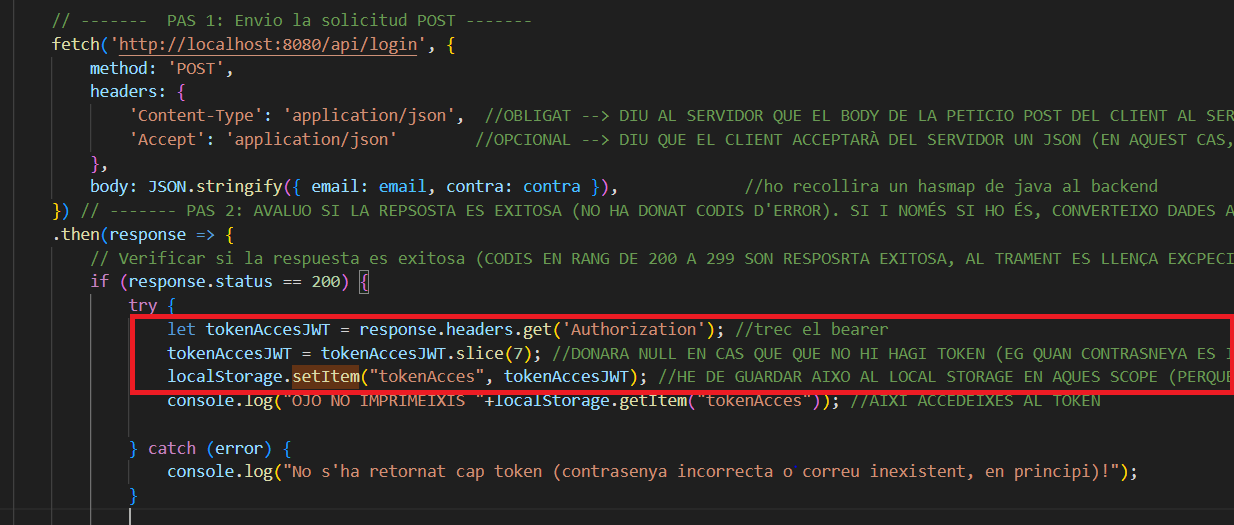
\includegraphics[width=1\textwidth]{img/jwtFetchLoginFront.png}
				
				\label{fig:figuraLoginFetch} 
			\end{figure}
			\FloatBarrier
			
			

			
			\section{desarrollo back-end (Spring Boot)}
			
				\subsection{Estructura de la aplicación}
				\label{sec:estructuraAplicacion}
				
				TO DO pom.xml application.properties, usuari, repository, service, controller.
				
				TO DO Parlar de les validacions i les anotacions 
				
				Parlar dels apartats de seguretat (segurity filter chain i JWT pero només de passada perque els mencionem despres)
				
				\subsection{Autenticacion y Autorización}
				
				\subsubsection{método utilizado: JWT}
				
				Para autenticar y autorizar a los usuarios no utilizaremos sesiones. Las sesiones, tal y como vimos en la asignatura de desarrollo web entorno servidor, requieren guardar un estado en el servidor (si tenemos 100 usuarios conectados necesitamos rastrear 100 personas en el servidor) y un identificador de sesión en una cookie segura con HttpOnly puesto a True guardada en el navegador de cada uno de los usuario conectados que lo identifica en relación al servidor.
				
				Sin embargo, existe un método de acceso por token más escalable que no requiere guardar sesiones en el servidor (es decir, es un método ``stateless'' o sin estado) con el que nos basta tener solamente la Cookie Segura para guardarlo y ya está. Es un token que está autocontenido: es decir, puede contener ya el ID de usuario, nombre de usuario, roles que luego permitirán dar permisos o no en el servidor para acceder a determinadas APIs o recursos, etc. En definitiva, con JWT tenemos una autenticación más eficiente y un control del acceso preciso (autorización) sin necesidad de almacenar sesiones en el servidor.
				
				
				A este sistema lo llamamos JSON Web Token (\texttt{JWT}) y toda la información que contiene está encriptada o \textbf{firmada digitalmente} con SHA256 mediante una clave privada que solo tenemos nosotros en el servidor. Esta clave es igual para todos los tokens que generemos: la firma digital que emana de esta clave estará embedida, por así decirlo, en cada uno de esos tokens y \textit{será inválida} si un atacante ha modificado el token y nos lo devuelve al servidor tratando de suplantar la identidad de algún usuario; con ello, el servidor rechazará la integridad del token y evitará que pueda acceder a recursos del usuario al que trata de suplantar.
				
				JWT no es perfecto, por supuesto. Una desventaja del JWT es que una vez puesta una fecha de expiración el desarrollador ya no la puede cambiar. En las sesiones del servidor se pueden extender las sesiones si se detecta actividad del usuario, acortarlas si pasa justo lo contrario o incluso cerrar la sesión de un usuario en remoto; pero con JWT no es posible: una vez creado el Token de acceso la fecha de actividad del mismo no se puede modificar (porque no puedes invalidar un token ya existente!). La solución que se propone con JWT es tener, por lo tanto, dos tokens almacenados en el cliente: el ``access token'' que es el que permite autenticar y autorizar, del que hemos hablado hasta ahora; y el ``refresh token'', que tiene la función de validar si el token de refresco sigue siendo válido con el servidor, y si lo es, entonces permite que el servidor emita un nuevo ``access token'' para el usuario. De este modo el usuario no deberá estar generando nuevos tokens constantemente. En este trabajo solo utilizaremos ``access tokens'' y ya está. Cuando un usuario se desloguee, lo que haremos será borrar el access token de la cookie, local storage o session storage y ya está.
			
				 
				 \noindent En resumen, \texttt{las ventajas} que tiene JWT vs uso de sesiones (assumiendo que tanto JWT como SESSID se guarden en una cookie segura) son las siguientes:
				 
					\begin{tabular}{l}
						\textbf{- No depende del almacenamiento en el servidor} \\
						\textbf{- Firmado digitalmente} \\
						\textbf{- Mayor control sobre el acceso} \\
						\textbf{- Mayo descentralización} \\
						\textbf{- Menos carga para el servidor}
					\end{tabular}
									 
				   \noindent Y la \texttt{desventaja} más evidente que tiene JWT, es, en nuestra opinión, su complejidad\footnote{Se puede ver una tabla de diferencias más en profunidad, especialmente en materia de seguridad en el anexo \ref{sec:anexo_JWTvsSESSIONS})}, pues para tener un buen equilibrio entre facilidad de uso y seguridad es necesario almacenar los tokens en el cliente para conseguir que uno se renueve (el token de aceso y el de refresco, como comentamos):
				  
				  \begin{tabular}{l}
					 \textbf{- Caducidad de tokens irrevocable}\\
					 \textbf{- Renovación de tokens de acceso con uno de refresco}
				  \end{tabular}
				 

				
				
				
				\subsubsection{¿Qué compone un JWT?}
				
				\noindent El JWT se compone de tres partes. \textbf{los headers}, \textbf{el payload} y \textbf{la signatura}. En la página \href{https://jwt.io/}{https://jwt.io/}, como veremos después, se puede ver si los tokens son válidos, observar su estructura interna, etc. \cite{jwtio}. A saber:
				

				\begin{itemize}
					\setlength{\itemsep}{-.5em}
					\item 				\textbf{Los headers}: Aportan información sobre el algoritmo que lo encriptó.
					\item 				\textbf{El payload}: Es donde está la información que nos interesa del token: el sujeto que lo generó (``sub''), el momento en que se generó el toquen (``iat'', o ``issued at'') y la fecha de expiración (``exp'' o ``expiration time''). También podemos tener ahí otros pares clave valor que podremos querer definir, por ejemplo, que contengan el id del usuario y sus roles o permisos que son los que nos permitirán dejar que un determinado usuario pueda consultar o no ciertos recursos.
					
					\item \textbf{La signatura}: Es la parte que garantiza la integridad del token y evita que sea alterado por terceros. Se genera aplicando un algoritmo de hash (en nuestro caso el SHA256) a la combinación del header y el payload, junto con la clave secreta que solo conoce el servidor (es lo que permetirá al servidor rechazar el token si no es válido -i.e. ha sido manipulado).
				\end{itemize}
				
				Podéis observar estas tres partes en colores en la figura \ref{fig:jwtioMostraPayload} que veremos después.
				
				
				

				

				
				
				\subsubsection{Implementación de JWT en java SpringBoot}
				\label{sec:implementacionJWTjava}
				Para poder implementarlo añadimos la dependencia \textbf{jjwt} en \texttt{pom.xml} que es la que nos permite definirlo.
				
				
				\begin{lstlisting}[language=XML, basicstyle=\ttfamily\small, keywordstyle=\color{red}]
					
	<dependency>
		<groupId>io.jsonwebtoken</groupId>
		<artifactId>jjwt</artifactId>
		<version>0.12.6</version>
	</dependency>
					
				\end{lstlisting}
				
				
		En el proyecto se han creado tres clases dentro de sus respectivos archivos en la ruta \texttt{src/main/java/} \texttt{miApp.app/seguretat/jwtseguretat} denominadas:
		
		\begin{itemize}
			\setlength{\itemsep}{-.4em}
			\item \textbf{JwtUtil}
			\item \textbf{AccessToken}
			\item \textbf{RefreshToken}
		\end{itemize}
		  
		
		En la clase \textbf{JwtUtil} hemos creado un método que obtiene las \textit{claims} (pares clave valor que contienen la carga útil de un JWT) y en el constructor hemos creado la definición de una clave privada con la que derivar todas las instancias que hagamos de esa clase -es decir, todos los tokens que se cifren con esa contraseña-. De esta clase hemos heretado las otras dos: La subclase que nos genera el \textit{token de acceso}, \textbf{AccessToken}; y la que nos genera el \textit{token de refresco}, \textbf{RefreshToken}. A continuacion podéis, de estas tres, la más importante: 
		
		

		
\begin{lstlisting}[language=Java, basicstyle=\ttfamily\footnotesize, keywordstyle=\color{magenta}]
				
@Component
public class AccessToken extends JwtUtil {
	
  private static int tExpM; //minuts per a exprirar el token
	
  public AccessToken() {this.tExpM = 10;}
	
  //FINALITAT: Generar un JWT d'acces.
  public String genera(String correu, int idUsuari, byte permisos) {
	Map<String, Object> dadesExtraApayload = new HashMap<>();
	dadesExtraApayload.put("permisos", permisos);
	dadesExtraApayload.put("idUsuari", idUsuari);
		
	return Jwts.builder()
	 .setClaims(dadesExtraApayload) //dades customitzades
	 .setSubject(correu)            //guardo nom subjecte (clau "sub")
	 .setIssuedAt(new Date())       //data creacio (clau "iat" payload)
	 .setExpiration(new Date(System.currentTimeMillis() + (tExpM*60*1000)))
	 .signWith(SignatureAlgorithm.HS256, clauSecreta.getBytes())
	 .compact();
}


\end{lstlisting}
		
		
		
		Con la función \textbf{genera()} de la clase AccessToken arriba mostrada, y con los parámetros necesarios que serán necesarios para autorizar (idUsuari) y autenticar (permisos), podemos generar un token de acceso en ``accesJWT'':
		
		
		
\begin{lstlisting}[language=Java, basicstyle=\ttfamily\footnotesize, keywordstyle=\color{magenta}]

AccessToken accessToken = new AccessToken();
String accesJWT = accessToken.genera(
	"santo@gmail.com",  //campoSub
	2, //idUsuari
	1  //permisos
);


\end{lstlisting}
		
		Si vemos la figura \ref{fig:jwtioMostraPayload} que tenemos a continuación, veremos en la mitad izquierda un token de acceso generado por la función anterior. Fijémonos que internamente ese token está estructurado en las tres partes de la parte derecha de la imagen, siendo la payload la más importante:
		
	
			\setlength{\belowcaptionskip}{3pt}
			\FloatBarrier
			\begin{figure}[H]
				\centering
				\caption{Decodificación de un token de acceso generado con la función genera de la clase AccessToken mediante \href{https://www.jwt.io}{jwt.io}. La Payload con las claims en flecha verde.}
				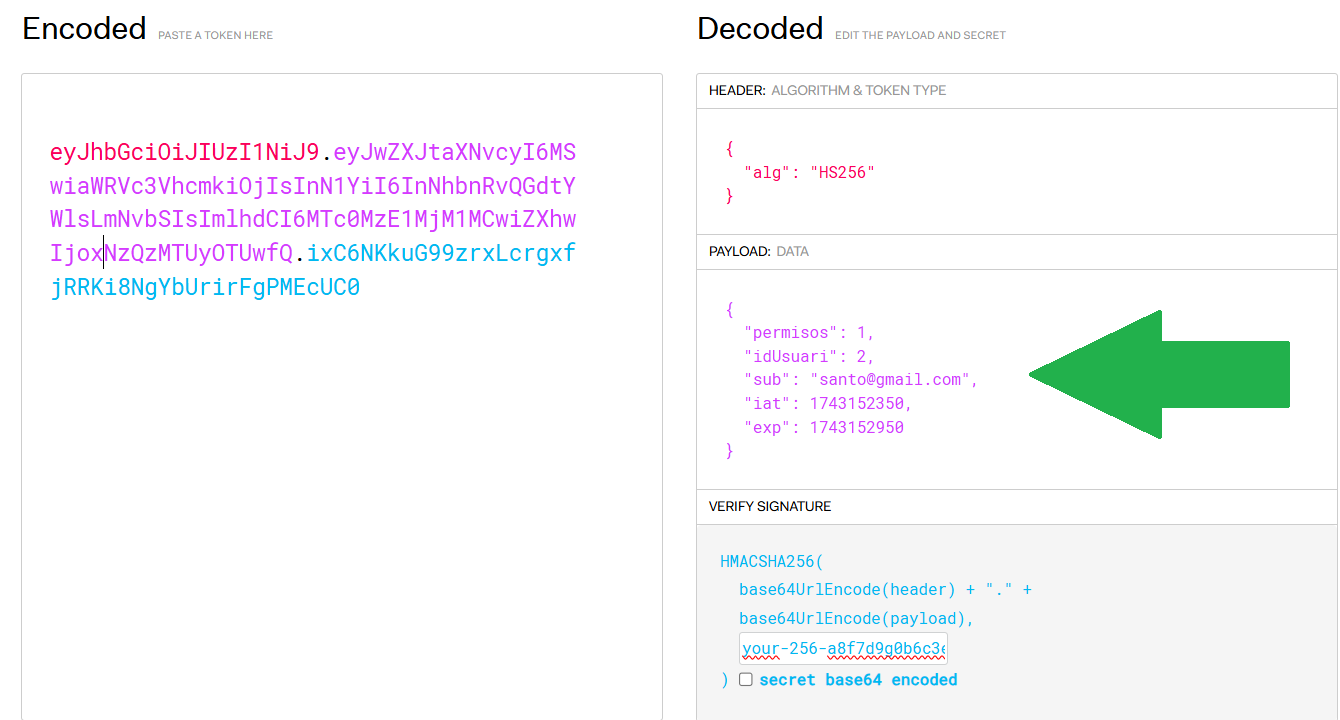
\includegraphics[width=1\textwidth]{img/jwtio_mostra_payload.png}

				\label{fig:jwtioMostraPayload} 
			\end{figure}
			\FloatBarrier

		
\begin{lstlisting}[language=Java, basicstyle=\ttfamily\footnotesize, keywordstyle=\color{magenta}]
			
		
		{
		    "permisos": 1,
		    "idUsuari": 2,
		    "sub": "santo@gmail.com",
		    "iat": 1743152350,
		    "exp": 1743152950
		}
			
\end{lstlisting}
		
		
		
		
		
		Al generar las tres clases hemos utilizado herencia porque la clave privada es la misma para ambos tipos de token (tanto el de acceso como el de refresco), mientras que los métodos para generar cada uno de los dos tipos de token cambian. En StackOverflow existe un debate para ver si hay que tener una clave privada distinta para cada tipo de token, por si el lector está interesado \cite{stackoverflow_jwt_refresh_token_secret}. Después de ver la entrada en stackOverflow Se ha optado por compartir claves para ambos tipos.
		
		
		En la clase \textbf{JwtUtil} tenemos una función denominada \texttt{getClaims()} que es la que utilizaremos en el Service de nuestra aplicación para poder autenticar y autorizar usuarios. Las tres clases pueden ser consultadas en el anexo \ref{sec:anexoCreacionYverificacionJWT} o en el GitHub del proyecto (\href{https://github.com/blackcub3s/mercApp/blob/main/APP%20WEB/__springboot__produccio__/app/src/main/java/miApp/app/seguretat/jwt}{link}). Se recomienda encarecidamente al lector optar por esta última opción\footnote{Al poner las tres clases en anexo se omitieron las funciones main donde se testeaban las funciones de creación de tokens con control de excepciones, comentarios e imports por falta de espacio en el DIN A4.}.
		
		\subsubsection{Enviar por primera vez el Access Token hacia el front-end}
		\label{sec:enviarPorPrimeraVezAccesTokenDESDEBACKEND}
		
		Cuando el usuario consigue poner la contraseña correcta en la página del front-end \textbf{pas2C\_login.html} se manda de vuelta del back-end (desde el controlador de endpoint \texttt{/login}) hasta el front-end en el localStorage (¡por ahora lo hemos hecho así por simplicidad, pero en producción debería estar en una cookie segura!).
		
		La parte de recepción del token en el front-end y de su manejo podéis encontrarla en el apartado \ref{sec:recibirAccesTokenENFRONTEND}

		
		
		
		
		
		
		\textbf{TO DO: Referenciar endpont login springboot (que cal millorar)}
		
		\subsubsection{Recibir el JWT enviado por el front-end, interpretarlo desde el back-end y con ello securizar un endpoint de la API desde el back-end}
		
		Después de crear las tres clases en Java de las que hemos hablado en el apartado \ref{sec:implementacionJWTjava} anterior y haber mandado el token de acceso al front, podemos empezar a 
		implementar la protección de endpoints con JWT. Asumamos que nos llega un token de acceso en una solicitud HTTP de un usuario que ya acaba de recibir el token y quiere acceder al dashboard de visualización (a través de la heather ``Authorization'') (\texttt{'usuaris/{id}/endpoinTikets'}) (ver subseccion \ref{sec:estructuraAplicacion}, en ControladorUsuari.java). 
		
		En javascript puro, desde el cliente, esta solicitud HTTP la pondríamos conseguir de la función fetch(), poniéndole uno de los pares clave valor con el inicio ``Bearer'' (por convenio) tal que así:
		
				
\begin{lstlisting}[language=Java, basicstyle=\ttfamily\footnotesize, keywordstyle=\color{magenta}]

fetch("'http://localhost:8080/usuaris/{id}/endpointTikets'", {
	method: "GET",
	headers: {
		"Content-Type": "application/json",
		"Authorization": "Bearer "+tokenJWT;
	},
	...
}
\end{lstlisting}
		
		 Queremos conseguir que ese endpoint permita en cada solicitud \textbf{Autenticarlo}, es decir, determinar que dice ser quien es mediante el hecho de encontrar en el token verificado su idUsuari correspondiente (y acceder a la información de sus tickets); y a su vez \textbf{Autorizarlo}, es decir, dar acceso a ese usuario a los recursos a los que se le permita acceso.
		
		 Estos dos pasos irán en función del valor de la variable que haya emanado de la base de datos al conceder el token mediante \textit{idUsuari} para el caso de la \textbf{Autenticación} -ver \href{https://github.com/blackcub3s/mercApp/blob/b01cec515bb9af27a1faa24258abb4313ef275cd/APP%20WEB/__springboot__produccio__/app/src/main/java/miApp/app/Usuaris/model/Usuari.java#L30}{linea github}-, y de la variable \textit{permisos} del model de la @Entity class Usuari - ver \href{https://github.com/blackcub3s/mercApp/blob/b01cec515bb9af27a1faa24258abb4313ef275cd/APP%20WEB/__springboot__produccio__/app/src/main/java/miApp/app/Usuaris/model/Usuari.java#L42}{linea github}- para el caso de la \textbf{autorización}). Para ello hay \textbf{tres} pasos que debemos implementar dentro del back-end de SpringBoot:
		
		
		
		
		\begin{itemize} 
			\setlength{\itemsep}{-1.5em}
			\item \textbf{PASO 1:} Extraer la información del usuario autenticado desde \textit{el payload} del token JWT entrante. Para ello crearemos un \textbf{Filtro de Autenticacion} dentro de \texttt{FiltreAutenticacio.java}\\
			\item \textbf{PASO 2:} Configurar el contexto de seguridad para que Spring Security reconozca los permisos dentro de  \texttt{ConfiguracioSeguretat.java}. \\ 	
			\item \textbf{PASO 3:} Aplicar restricciones con \textbf{@PreAuthorize} en cada \textit{endpoint} que queramos proteger en el controlador dentro \texttt{UsuariControlador.java}
		\end{itemize}
		

		\paragraph{PASO 1: Extracción del payload}
		Esta parte del código está llena de boilerplate. La clase \texttt{FiltreAuntenticacioJwt.java} extiende de OncePerRequestFilter \cite{oncePerRequestFilter}, que como dice el propio nombre de ala clase implementa un filtro que se desarrollará una vez por cada petición al servidor.
		
		\paragraph{PASO 2: Configuración contexto seguridad}
		
		\paragraph{PASO 3: restricciones en el controlador}
		
		

		
	\section{desarrollo back-end (microservicio con Python)}
		
		
	\chapter{Evaluación y Conclusiones Finales} %OBLIGAT
	

	
	
	
	

	
	
	
	
	
	
	
	
	
	
	
	
	
	
	
	
	
	
	
	
	
	
	
	
	
	
	
	
	
	
	
	
	
	
	
	
	
	
	
	
	\chapter{ANEXO}
	\label{chap:anexo} % Esta es la etiqueta de referencia
		
			
		\section{Flujo de trabajo habitual en git}
		\label{sec:anexoFlujoGit}
		
\begin{lstlisting}[language=bash, basicstyle=\ttfamily\small]
	


# trabajamos con el proyecto y se introduce
# en el staging area
git add -A 

# creamos rama para aglutinar los cambios
git branch backEnd

# cambiamos a la rama que acabamos de crear
git checkout backEnd

# guardamos los cambios como nodos dentro de
# la rama con la que desarrollamos.	
git commit -m "commit 1"  	
git commit -m "commit 2"
# [...]
git commit -m "commit n"

#cambiamos a rama main local y luego integramos cambios
git checkout main
git merge backEnd

#Subimos los cambios al repo remoto
git push origin main 

	
\end{lstlisting}
		
	
\pagebreak

		
		
		\section{Diferencias de seguridad: JWT vs SESSID en cookies seguras}
		\label{sec:anexo_JWTvsSESSIONS}
						
			\FloatBarrier
			\begin{table}[h]
				\centering
				\begin{tabular}{|p{4cm}|p{5cm}|p{5cm}|}
					\hline
					\textbf{Característica} & \textbf{JWT en cookies seguras} & \textbf{Session ID en cookies seguras} \\
					\hline
					\textbf{Seguridad contra XSS} & Más seguro si la cookie tiene \texttt{HttpOnly} y \texttt{Secure}, ya que no es accesible desde JavaScript. & Más seguro si la cookie tiene \texttt{HttpOnly} y \texttt{Secure}, ya que no es accesible desde JavaScript. \\
					\hline
					\textbf{Seguridad contra CSRF} & Puede ser vulnerable si la cookie no tiene \texttt{SameSite=Strict}. & Menos vulnerable si la cookie tiene \texttt{SameSite=Strict}. \\
					\hline
					\textbf{Estado en el servidor} & Stateless (no hay estado en el servidor, el JWT contiene toda la información). & Stateful (el servidor mantiene una sesión activa asociada con el Session ID). \\
					\hline
					\textbf{Escalabilidad} & Mejor escalabilidad porque no requiere almacenamiento de sesiones en el servidor. & Menos escalable, ya que el servidor debe manejar las sesiones activas. \\
					\hline
					\textbf{Expiración y revocación} & Difícil de revocar antes de que expire, a menos que se implemente una lista negra en el servidor. & Fácil de invalidar eliminando la sesión en el servidor. \\
					\hline
					\textbf{Uso con JavaScript} & No accesible desde JavaScript si la cookie tiene \texttt{HttpOnly}. & No accesible desde JavaScript si la cookie tiene \texttt{HttpOnly}. \\
					\hline
				\end{tabular}
				\caption{Comparación de seguridad entre JWT y Session ID almacenados en cookies seguras con HttpOnly=True.}
				\label{tab:jwt_vs_session}
			\end{table}
			\FloatBarrier
	
		\pagebreak
		
		
		\section{Clases para crear y verificar JWTs}
		\label{sec:anexoCreacionYverificacionJWT}
	
	
\subsection{Clase JWT}


\begin{lstlisting}[language=Java, basicstyle=\ttfamily\tiny, keywordstyle=\color{magenta}]
	
//NO INSTANCIEM AQUESTA CLASSE MAI. LA FEM ABSTRACTA
@Component
public abstract class JwtUtil {
	
	//es la clau privada de 256 bits com a minim per encriptar el token (tant el d'acces com el de refresh)
	//veure debat http://bit.ly/3RmBGIK
	protected static String clauSecreta;
	
	public JwtUtil() {
		this.clauSecreta = "a8f7d9g0b6c3e5h2i4j7k1l0m9n8p6q3r5s2t1u4v0w9x8y7z";
	}
	
	//METODE QUE PARSEJA EL TOKEN JWT COMPLET. VERIFICA LA FIRMA I EXTRAU LES CLAIMS (parells clau valor en el payload).
	protected Claims getClaims(String token) {
		return Jwts.parser()
		.setSigningKey(clauSecreta.getBytes())
		.build()
		.parseClaimsJws(token)
		.getBody();
	}
	
}






\end{lstlisting}


				

\subsection{Clase Refresh Token}

\begin{lstlisting}[language=Java, basicstyle=\ttfamily\tiny, keywordstyle=\color{magenta}]

@Component
public class RefreshToken extends JwtUtil {
	
	private static int tExpDies;
	
	public RefreshToken() {this.tExpDies = 7;}
	
	// FINALITAT DEL METODE: Refrescar el token d'acces que genera generaAccesToken().
	public String generaRefreshToken(String correu, int idUsuari) {
		Map<String, Object> dadesExtraApayload = new HashMap<>();
		dadesExtraApayload.put("idUsuari", idUsuari);
		//posar mes dades al payload si es necessari
		
		return Jwts.builder()
		.setClaims(dadesExtraApayload) //dades customitzades
		.setId(String.valueOf(UUID.randomUUID().toString())) //id unic per a token. Per traSSSabilitat
		.setSubject(correu)           //guardo nom subjecte (dins "sub")
		.setIssuedAt(new Date())      //data creacio
		.setExpiration(new Date(System.currentTimeMillis() + tExpDies*86400*1000))  //expiracio
		.signWith(SignatureAlgorithm.HS256, clauSecreta.getBytes())
		.compact();
	}
}

\end{lstlisting}


\subsection{Clase Access Token}
\begin{lstlisting}[language=Java, basicstyle=\ttfamily\tiny, keywordstyle=\color{magenta}]

@Component
public class AccessToken extends JwtUtil {
	
	private static int tExpM; //minuts per a exprirar el token
	
	public AccessToken() {this.tExpM = 10;}
	
	//FINALITAT: Generar un JWT d'acces.
	public String genera(String correu, int idUsuari, byte permisos) {
		Map<String, Object> dadesExtraApayload = new HashMap<>();
		dadesExtraApayload.put("permisos", permisos);
		dadesExtraApayload.put("idUsuari", idUsuari);
		
		return Jwts.builder()
		.setClaims(dadesExtraApayload) //dades customitzades
		.setSubject(correu)            //guardo nom subjecte (clau "sub")
		.setIssuedAt(new Date())       //data creacio (clau "iat" payload)
		.setExpiration(new Date(System.currentTimeMillis() + (tExpM*60*1000)))
		.signWith(SignatureAlgorithm.HS256, clauSecreta.getBytes())
		.compact();
	}
}
	
				
\end{lstlisting}
	

	
		\section{CODIGO 5}
		\label{sec:KLNASQOW}
	

		


		
	% Bibliografía (\chapter(6. Bibliograifa) como implicito)
	\addcontentsline{toc}{chapter}{7. Bibliografía} 
	\bibliographystyle{plain}  % Estilo de bibliografía
	\bibliography{referencias} % Nombre del archivo .bib  extensión
	
		
	

	\endgroup
\end{document}
